\documentclass{ttithesis}

\usepackage{amsmath}
\usepackage{graphicx}
\usepackage{scrextend}
\usepackage{setspace}
\usepackage{color}
\usepackage{tabularx}
\usepackage{csvsimple}
\usepackage{nameref}

\newcommand{\fixme}[1]{\textbf{\colorbox{black}{\textcolor{red}{#1}}}}
\newcommand{\unicode}[1]{\textbackslash u#1}
\newcommand{\fullref}[1]{\ref{#1}\nameref{#1}}
\newcommand{\vc}[1]{\mathbf{#1}}
\newcommand{\rival}{従来手法\cite{fujitani15}}
\newcommand{\nn}{ニューラルネットワーク}


\title{文書・文間及びカテゴリ間の関係を考慮した\\レーティング予測}
\author{12056\hspace{16ex}外山洋太}
\date{平成28年 2月}
\laboratory{知能数理研究室}



\begin{document}

\section{序論}

企業において商品の評判分析のためのレビューの評判分類は重要な問題である。
何万件という大量のレビューデータを人手で処理することは難しく、
計算機による自動化が望まれる。
その中で商品を複数のカテゴリにおいて分類をする問題がある。
カテゴリとは、宿泊施設のレビューを例にすると、サービス、立地、食事等の
レーティングが付けられる各項目のことである。
この問題に関する従来手法\cite{fujitani15}は、文間の関係性を考慮しておらず、
カテゴリ間については考慮しているものの深い関係性を捉えることができていない。

近年、その評判分類において、ニューラルネットワークを用いた手法
\cite{nal14,rie14,duyu15}が
提案されており、従来の手法を上回る正答率を達成している。
ニューラルネットワークを分類問題に用いる利点はまず
層の数を増やすことによって入力の深い繋がりを考慮できることである。
例えば、文毎の素性を入力とすれば文間の関係性を捉えることができる。
さらに、多カテゴリの分類問題においてはカテゴリ間の関係性を捉えた分類が
実現できる。
しかし、評判分類に関する多くの研究は1つのカテゴリにおける二値分類問題を
対象としている。

文や文章の意味表現の学習手法として、単語と文章の分散表現を同時に学習する
パラグラフベクトル\cite{quoc14}がある。
これは評判分類問題に対して優れた性能を示している。
しかし、文書全体にパラグラフベクトルを用いた場合、
分類時に文の位置関係を考慮できない。

本研究は、複数カテゴリにおける評判分類について、
文書及び文間の関係とカテゴリ間の関係を同時に考慮した分類を実現することを
目的とする。

提案手法では、パラグラフベクトル\cite{quoc14}によって
生成された各レビューの文書ベクトルと文ベクトルを
ニューラルネットワークによる分類器において分類しレーティング予測を行う。
楽天トラベルのデータセットを用いた実験において、
提案手法は従来手法\cite{fujitani15}に対して約2pp上回る正答率を
示した。
レーティングの平均二乗誤差(RMSE)を元にした評価基準では、
従来手法\cite{fujitani15}において弱点となっていたカテゴリについて
それを上回る結果を示した。

\section{関連研究} \label{sec:RelatedResearch}

多カテゴリにおけるレーティング予測に関する従来研究、
及び、提案手法に関連した研究や技術について述べる。
はじめに提案手法で用いているパラグラフベクトルと深層学習について述べる。
次に、レーティング予測について、多カテゴリのものを対象とした従来手法と
ニューラルネットワークを用いた手法について述べる。
最後に、その他本研究で利用した研究や技術について述べる。


\subsection{パラグラフベクトル}

パラグラフベクトルは、文や文書といった大きな単位の言語表現の意味表現を
学習する手法である。
これは、Continuous BOW (CBOW)またはSkip-gram\cite{yoshua03}という
単語の意味表現の学習手法を応用した手法である。
ここではCBOWを応用したDistributed Memory model of Paragraph Vectors (PV-DM)
について説明する。
PV-DMはBOWと異なり、単語の並び順を考慮した文や文書の分散表現を
生成することができる。

\begin{figure}
  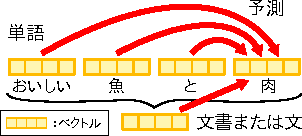
\includegraphics[0.5]{fig/paragraph_vector_v2.pdf}
  \caption{パラグラフベクトルの学習の概略}
  \label{fig:ParagraphVector}
\end{figure}

以下に具体的なアルゴリズムを示す。
ここでは文書の意味表現を学習する場合について考える。
学習の概略を図\ref{fig:ParagraphVector}に示す。
まず、意味表現を学習する対象となる文書に含まれる単語を
初めから一つずつ読んでいく。
その際、現在の単語及びその周辺の単語、現在の文書について、
式\ref{eq:ParagraphVector}に示す目的関数$L$を最大化するように
各パラメータの学習を行う。
\begin{gather} \label{eq:ParagraphVector}
  L = \sum_d L_d \\
  L_d = \frac{1}{T} \sum^{T}_{t = k} \log p(w_t | w_{t-k}, ..., w_{t-1}),
     \nonumber \\
  p(w_t | w_{t-k}, ..., w_{t-1}) = \frac{e^{y_{w_t}}}{\sum_{w'} e^{y_{w'}}},
    \nonumber \\
  y = b + Uh(w_{t-k}, ..., w_{t-1}, d; W, D) \nonumber
\end{gather}
ここで、$L_d$は文書$d$の目的関数である。
$w_i$は単語、$W$は全ての単語の分散表現を表す行列、
$D$は全ての文書の分散表現を表す行列である。
$k$はウィンドウサイズ、$T$は現在の文書に含まれる単語数である。
ある単語の周辺を表す区間をウィンドウという。
$p$はsoftmax関数により正規化された、文脈から現在の単語が導かれることの
尤度である。
$p$を構成する$y$は現在の単語とウィンドウ内の単語及び現在の文書から導出される。
$h(w_{t-k}, ..., w_{t-1}, d; W, D)$は単語$w_{t-k}, ..., w_{t-1}$のベクトルと
文書$d$のベクトルをそれぞれ$W$と$D$から取り出し結合して返す関数である。

PV-DMによって生成したレビューの文書のベクトルを
ニューラルネットワークによって分類することで、
レーティング予測においてBOW等より高い正答率が得られることが示されている。
しかし、文書全体にパラグラフベクトルを用いる場合、文間の関係が
予測時に考慮できない。


\subsection{深層学習}

深層学習とは、多層のニューラルネットワークを用いた
機械学習の手法の総称である\cite{takayuki15}。
以下には、その内ニューラルネットワークの正則化を行うための2つの手法、
ドロップアウトと重み減衰について述べる。
また、提案手法と直接関係がないが、関連するニューラルネットワークによる
レーティング予測の手法\cite{nal14,rie14,duyu15}で用いられているため、
畳み込みニューラルネットワークについても説明する。

ドロップアウトとは、ニューラルネットワークにおける層のニューロンの数を
一時的に減らすことによって正則化を行う方法である。
ある層に対してドロップアウトを行うには、その層が持つニューロンの出力値を
確率的に0とする。
%また、出力値が0となったニューロンに対する重みの勾配は0となるため、
%そのニューロンに対する重みはその学習回において更新されない。
これを各学習回で行うことで、ニューラルネットワーク全体を学習する。

次に、重み減衰について説明する。
重み減衰とは、ニューラルネットワークの各重みをその大きさに応じて
学習回毎に減少させる正則化の手法である。
重み減衰を行うためには、ニューラルネットワークの最小化すべき目的関数に対して
各重みの2ノルムを足し合わせる。
式\ref{eq:NNObjectiveWithWeightDecay}に、重み減衰を適用した目的関数$L'$示す。
\begin{gather} \label{eq:NNObjectiveWithWeightDecay}
  L' = L + \frac{\lambda}{2} \sum_{\mathbf{w}} {|\mathbf{w}|}^2
\end{gather}
ここで、$L$はニューラルネットワークの重み減衰を適用していない目的関数である。
$\mathbf{w}$はニューラルネットワークの各層における重みである。
$\lambda$は重みの減衰率である。
式\ref{eq:NNObjectiveWithWeightDecay}により、
ニューラルネットワークのある層の重み$\mathbf{w}$に対する
更新式は式\ref{eq:WeightUpdateEquation}のようになる。
\begin{gather} \label{eq:WeightUpdateEquation}
  \mathbf{w} \leftarrow \mathbf{w} - \frac{\partial L}{\partial \mathbf{w}}
                                   - \lambda \mathbf{w}
\end{gather}
ここで、$a \leftarrow b$は変数$a$の値をそのときの式$b$の値で
更新することを示す。
ただし、全結合層のバイアス等では一般に重み減衰を行わない。
なぜならば、そのような重みの値は場合によって大きい値を
取る必要があるためである。

最後に、畳み込みニューラルネットワークについて説明する。
畳み込みニューラルネットワークとは、畳み込み層とプーリング層を用いた
ニューラルネットワークである。
一般に、畳み込み層とプーリング層は交互に配置される。
畳み込みニューラルネットワークは入力の局所的な特徴を抽出することができる。
また、畳み込みニューラルネットワークは元々画像認識に応用されていた手法であり、
その入力は複数のチャネルを持つことがある。
チャネルとは、画像でいうRGBの各色のことである。
例として、畳み込みニューラルネットワークの入力をRGB画像とした場合、
それは(チャネル)×(画像の幅)×(画像の高さ)の3次元行列で表される。
以下では、複数チャネルを持つ画像に対して畳み込みニューラルネットワークを
適用する場合の畳み込み層とプーリング層について説明する。

畳み込み層とは、前の層の各ニューロンが
次の層のニューロンの内、位置の近いものとしか結合しないように
全結合層を単純化した層である。
具体的にはある$H \times H$の大きさを持つフィルタを考え、
それを畳み込み層の入力値に適用して値を出力する。
図\ref{fig:ConvolutionalLayer}にその概略を示す。
\begin{figure}
  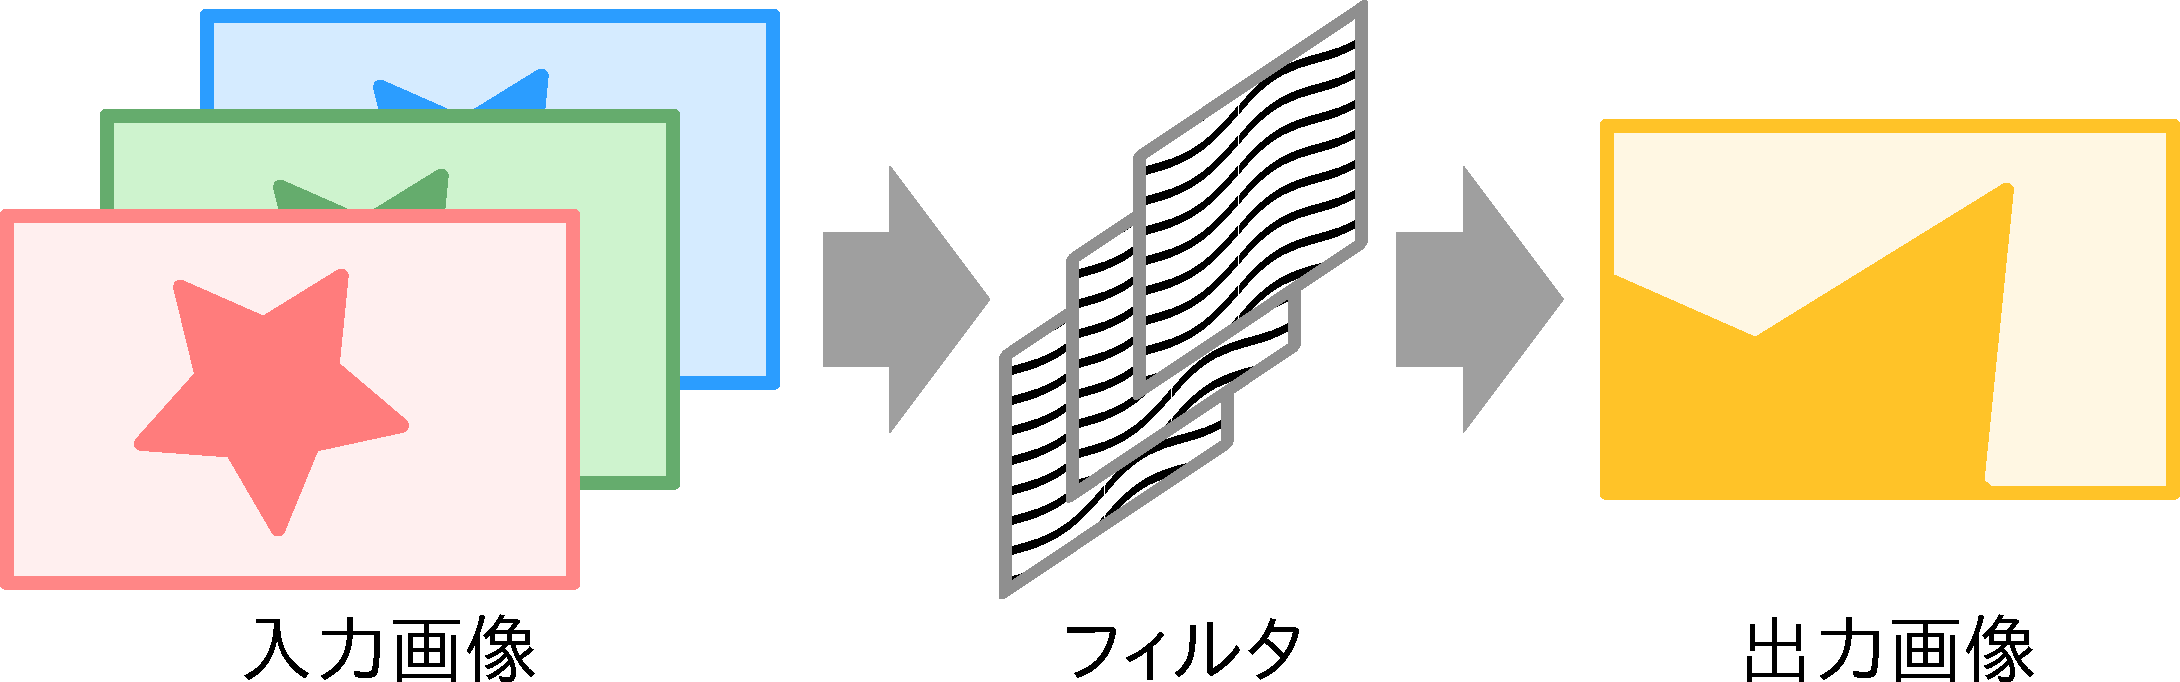
\includegraphics[0.7]{fig/convolutional_layer_with_one_filter.pdf}
  \caption{畳み込み層の概略}
  \label{fig:ConvolutionalLayer}
\end{figure}
式\ref{eq:ConvolutionalLayerFilter}に、畳み込み層のフィルタ$f$によって
処理された出力値$u_{fij}$を示す。
\begin{gather} \label{eq:ConvolutionalLayerFilter}
  u_{fij} = \sum^{C - 1}_{c = 0} \sum^{H - 1}_{p = 0} \sum^{H - 1}_{q = 0}
            z^{(l - 1)}_{c, i + p, j + q} h_{fcpq} + b_{fij}
\end{gather}
ここで、$z^{(l - 1)}_{c, i + p, j + q}$は、前の層$l - 1$の出力値である。
$H$はフィルタの幅である。
$h_{fcpq}$はチャネル$c$に対するフィルタ$f$の重みである。
$b_{fij}$はフィルタ$f$のバイアスである。
ただし、バイアスの値は位置によらず一つのフィルタ内で共有することが多い。
$(i, j)$は出力画像における位置である。
$(p, q)$はフィルタ$f$における位置である。
最終的な畳み込み層の出力値$z_{fij}$は$u_{fij}$の値に活性化関数を適用し
計算する。
\begin{gather} \label{eq:ConvolutionalLayerOutput}
  z_{fij} = \sigma(u_{fij})
\end{gather}
ここで、$\sigma$は活性化関数である。
実際の畳み込み層は複数のフィルタを持つことが多い。

次に、プーリング層とは入力画像の局所的な平均や最大値を取る層である。
これによって、入力画像における特徴の位置に関するノイズを緩衝できる。
式\ref{eq:PoolingLayer}に、平均プーリング層の出力値の位置$(i, j)$における
出力値$u_{cij}$を示す。
\begin{gather} \label{eq:PoolingLayer}
  u_{cij} = \frac{1}{H^2} \sum_{(p, q) \in P_{ij}} z_{cpq}
\end{gather}
ここで、$H$はプーリングする範囲の幅である。
$P_{ij}$は出力画像の位置によるプーリングの範囲であり、位置の集合で表される。
$c$はチャネルである。
$(i, j)$は出力画像における位置である。
$(p, q)$はあるプーリングの範囲$P_{ij}$における入力画像での位置である。


\subsection{レーティング予測}

商品レビューにおけるレーティング予測とは、レビューの文書から
そのレビューに対して実際にユーザが付与したレーティングを予測する問題である。
ここではレーティング予測に関する研究の内、まず本研究の従来研究である
藤谷ら\cite{fujitani15}の手法について説明する。
その後、深層学習を用いたレーティング予測の手法について説明する。

\subsubsection{隠れ状態を用いたホテルレビューのレーティング予測}

藤谷ら\cite{fujitani15}は複数のカテゴリにおけるレーティング予測に対して、
Multi-Instance Multi-Label learning for Relation Extraction (MIML-RE)
\cite{mihai12}モデルを用いた手法を提案している。
その手法では、レビュー内の各文毎に予測した隠れレーティングから
レビュー全体のレーティングを予測する。
図\ref{fig:FujitaniRelationsAmongRatingCategories}のように、
文毎のレーティングからレビュー全体のレーティングを予測する際の
カテゴリ間の繋がりを手動で変化させカテゴリ間の関係性を考慮している。
各文の素性にはBag Of Words (BOW)またはBag Of n-gramsを用いている。
藤谷ら\cite{fujitani15}は各文毎に隠れレーティングを予測することによって
0.4832の正答率が得られることを示した。
また、カテゴリ間の繋がりによって正答率が変化することを示した。

\begin{figure}
  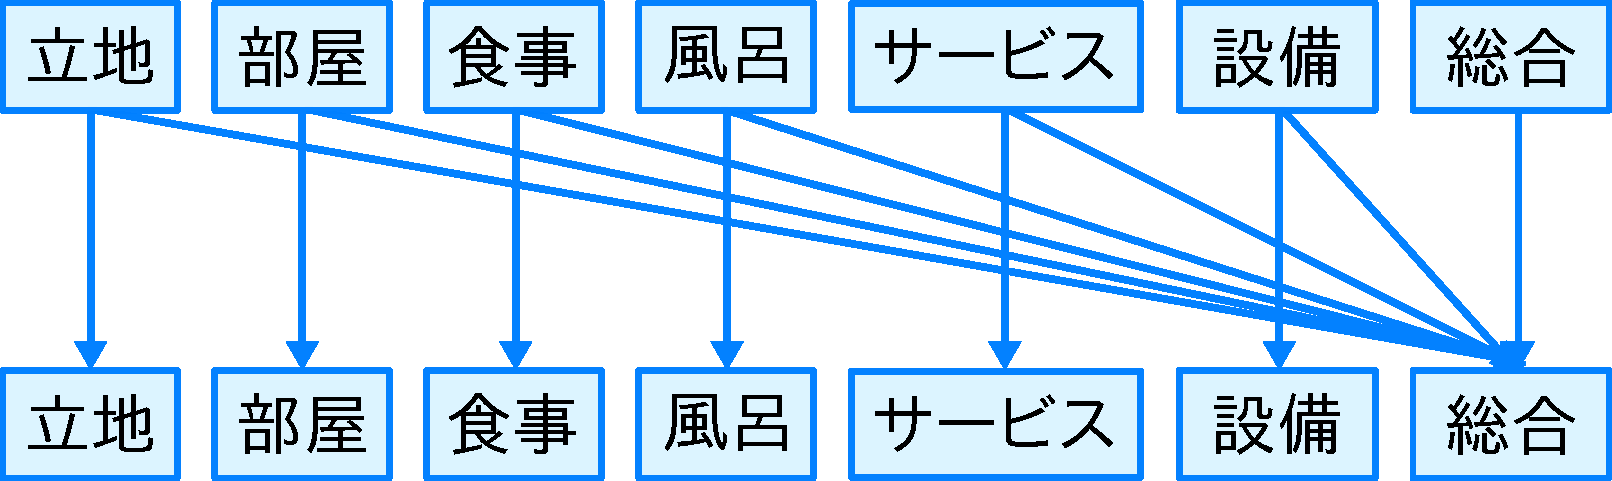
\includegraphics[0.5]
      {fig/fujitani_miml_relations_among_rating_categories.pdf}
  \caption{藤谷ら\cite{fujitani15}のモデルにおけるカテゴリ同士の繋ぎ方の例}
  \label{fig:FujitaniRelationsAmongRatingCategories}
\end{figure}

この手法では、文同士の位置関係を考慮しておらず、
カテゴリ間については考慮しているものの複雑な関係を考慮できていない。

\subsubsection{深層学習を用いたレーティング予測}

深層学習を用いたレーティング予測の手法が、Nalら\cite{nal14}、
Rieら\cite{rie14}、Duyuら\cite{duyu15}等によって提案されている。
これらの方法に共通するのは、単語や文の意味表現から
畳み込み\nn と全結合\nn を用いて予測を行うことである。
これらの手法では、まず、畳み込み層によって入力の局所的な特徴を捉える。
その後、畳み込み\nn から得られた文書全体の特徴を
全結合\nn の入力とし多値または二値分類を行う。
また、Nalら\cite{nal14}とDuyuら\cite{duyu15}の手法は
\nn のモデルの中にパラメータとして単語の意味表現を取り込んでいる。
これにより、特定の分類問題に対してそれらを最適化することができる。

Nalら\cite{nal14}は、単語の特徴から文の特徴を表現する、
分類や生成に適したモデルを提案している。
このモデルはDynamic Convolutional Neural Network (DCNN)と呼ばれる。
DCNNは畳み込み層とdynamic k-max pooling層、folding層、全結合層を
を組み合わせた多層の\nn である。
DCNNの畳み込み層はMax - Time Delay Neural Network (Max-TDNN)\cite{ronan08}
という文の意味を表現する\nn のモデルに基づいている。
Max-TDNNは、単語ベクトルの各次元毎に1次元フィルタを持った畳み込み層と、
その出力値に対して次元毎に最大値プーリングを行う層の2層と全結合層から
構成される\nn である。
Dynamic k-max pooling層は、プーリングの範囲からk個の最大値を
その順序を保持したまま取り出す層である。
このとき、$l$番目の畳み込み層の後のプーリングにおける$k$の値、$k_l$は
式\ref{KOfDynamicKMaxPooling}によって入力文毎に計算される。
\begin{gather} \label{KOfDynamicKMaxPooling}
  k_l = \max ( k_{top}, \lceil \frac{L - l}{L}s \rceil )
\end{gather}
ここで、$top$は最後の畳み込み層であり、
$L$はDCNNに含まれる畳み込み層の総数である。
$s$は入力文に含まれる単語の総数である。
また、folding層は入力となる行列を列方向に2行ずつ足し合わせる層である。
レーティング予測の実験において、Support Vector Machine (SVM)や
他の\nn を用いた手法と比較して、DCNNは高い正答率を示した。

Rieら\cite{rie14}はseq - Convolutional Neural Network (seq-CNN)と
bow - Convolutional Neural Network (bow-CNN)の2つの手法を提案している。
seq-CNNとbow-CNNの共通点は、文書の素性から畳み込み\nn と全結合\nn によって
レーティング予測を行うことである。
相違点は文書の素性である。
seq-CNNにおける文書の素性は、(語彙の大きさ)×(領域の大きさ)だけの
次元を持つベクトルからなる行列である。
図\ref{fig:SeqCNNTextFeature}のように、
文書はある単語数の領域毎に一定の単語数ずつずらしながら
分割され、行列に変換される。
ここで、領域とはある単語数を持つ文書内の区間のことである。
語彙の大きさだけの次元を持つベクトルは1つの単語を表すone-hotベクトルである。
(語彙の大きさ)×(領域の大きさ)だけの次元を持つベクトルは
それらを結合したベクトルである。
\begin{figure}
  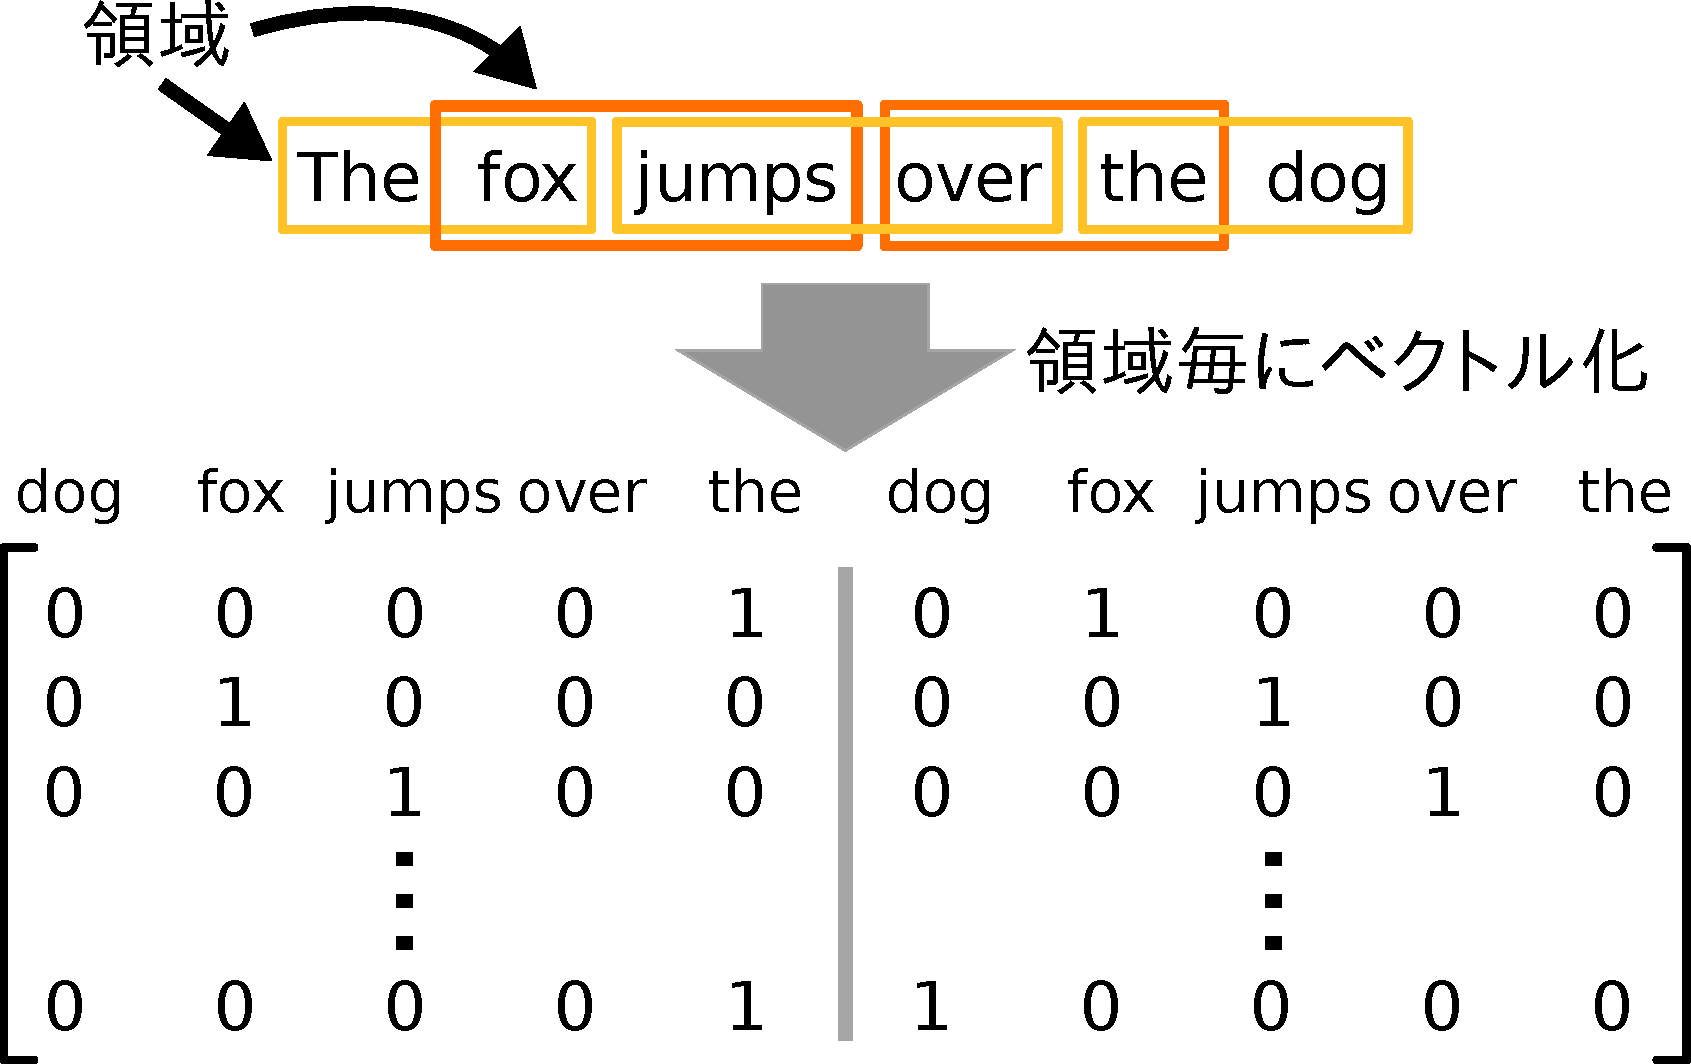
\includegraphics[0.6]{fig/seq_cnn_text_feature.pdf}
  \caption{seq-CNNにおける文書の素性の構成}
  \label{fig:SeqCNNTextFeature}
\end{figure}
一方、bow-CNNにおける文書の素性は、各領域毎のベクトルが
その領域のBOWであるような行列である。
実験では、Bag Of n-gramsによる文書の素性とSVMによる手法を含む他の手法に比べ、
seq-CNNとbow-CNNの畳み込み\nn の部分を並列に全結合\nn に結合したモデルが
より低い誤り率を示した。

Duyuらの手法は、単語ベクトルに対する畳み込み\nn に対し
ユーザ及び商品を表すパラメータを追加し拡張した手法である。
このモデルはUser Product Neural Network (UPNN)と呼ばれる。
Duyuらはレビューのデータセットに対して、
ユーザが付与するレーティングの一貫性、
商品が付与されるレーティングの一貫性、
ユーザが使用する単語の一貫性、
商品のレビュー文書に使用される単語の一貫性が
それぞれ成立することを検証した。
そこで、UPNNではこの4つの一貫性を表すパラメータがモデルに追加されている。
ユーザが使用する単語の一貫性、
商品のレビュー文書に使用される単語の一貫性はそれぞれ行列$U_k$と$P_j$で
表される。
ここで、$k$はユーザ、$j$は商品を表す。
これらの行列は畳み込みニューラルネットワークの入力となる各単語ベクトルを
式\ref{eq:UPNNProjectWord}のように写像する。
\begin{gather} \label{eq:UPNNProjectWord}
  \vc{w}' = \left[ \begin{array}{c} U_k \\ P_j \end{array} \right] \vc{w}
\end{gather}
ここで、$\vc{w}$は単語ベクトル、$\vc{w}'$は写像された単語ベクトルである。
次に、ユーザが付与するレーティングの一貫性、
商品が付与されるレーティングの一貫性はそれぞれベクトル$\vc{u}_k$と$\vc{p}_j$で
表される。
これらは畳み込み\nn の出力値と共に全結合\nn によって分類に利用される。
以上の行列$U_k$と$P_j$、及び、ベクトル$\vc{u}_k$と$\vc{p}_j$により、
4つの一貫性を考慮したレーティング予測を行うことができる。
実験では、UPNNが他の手法より高い正答率を示した。
また、UPNNと各一貫性を表現するパラメータをUPNNから取り除いたモデルを
比較することで、各パラメータが確かに正答率の向上に有効であることが示された。

以上の手法は、レビューの特徴を各観点から上手く考慮している一方で、
1つのカテゴリにおける多値または二値分類を対象としている。
よって、多カテゴリのレーティング予測において、これらの手法をカテゴリ毎に
適用しただけではカテゴリ間の関係を考慮することができない。


\subsection{形態素解析}

形態素解析とは、文等の文字列を形態素に分割する処理である\cite{hozumi06}。
ここで、形態素とは意味を持った言語の最小単位である。
日本語における形態素解析は、単語分割とその語形変化の解析に相当する。
以降、日本語の文字列を形態素解析する場合の単語分割について述べる。
単語分割の手法として、最長一致法と
%分割数最小法、
bi-gramマルコフモデルによる手法について説明する。

最長一致法では、解析すべき文字列を先頭から順に読み進めながら
解析結果となる単語を決定していく。
まず、文字列の現在の位置からの部分文字列が辞書内の単語と一致するか検査する。
次に、一致した単語の内、最も文字数の多いものを解析された単語として記録する。
最後に、その単語の文字数だけ文字列を読み進め、
再び現在の位置から始まる部分文字列に一致する単語を辞書で検索する。
これを繰り返していくことによって、文字列の終端まで形態素解析を行う。

これに対して、bi-gramマルコフモデルによる手法では単語のbi-gram確率を考え、
この積が文字列全体で最大となるように文字列を単語に分割する。
以下に最も適切な単語列$\hat{W}$を求める式を示す。
\begin{gather}
  \hat{W} = \text{argmax}_{W} P(W), \\
  P(W) = \sum^{n}_{i = 1} P(w_i | w_{i - 1}), \nonumber \\
  W = w_1, w_2, ... , w_n \nonumber
\end{gather}
ここで、$W$は元の文字列から分割された単語列であり、
$P(W)$はその単語列の同時確率である。
$w_i$は単語、$P(w_i | w_{i - 1})$は単語$w_i$と単語$w_{i - 1}$の
bi-gram確率である。


\subsection{Adam}

Adam\cite{diederik15}は確率的最適化のためのパラメータ更新のアルゴリズムである。
実験によって、Adamがニューラルネットワークに適用できること、及び、
パラメータをSGDやAdaGrad\cite{john12}より速く収束させることが
確かめられている。
式\ref{eq:AdamUpdate}にAdamによる目的関数$L$のパラメータ$\vc{w}$の
更新式を示す。
式\ref{eq:AdamUpdate}は、実際にはDiederikら\cite{diederik15}によって
示されている逐次的なアルゴリズムによって効率良く実装できる。
\begin{gather} \label{eq:AdamUpdate}
  \vc{w}_t = \vc{w}_{t - 1}
                 - \alpha \frac{\vc{m}_t}
                               {\sqrt{\vc{v}_t} + \epsilon}, \\
  \vc{m}_t = \frac{1 - \beta_1}{1 - {\beta_1}^t}
                 \sum^t_{i = 1} {\beta_1}^{t - i} \vc{g}_i, \nonumber \\
  \vc{v}_t = \frac{1 - \beta_2}{1 - {\beta_2}^t}
                 \sum^t_{i = 1} {\beta_2}^{t - i} {\vc{g}_i}^2, \nonumber \\
  \vc{g}_i = \frac{\partial L_i}{\partial \vc{w}_i} \nonumber
\end{gather}
ここで、$\vc{w}_t$は更新回数$t$におけるパラメータ$\vc{w}$を表す。
$\vc{m}_t$と$\vc{v}_t$は更新回数$t$における
パラメータ$\vc{w}$の一次・二次モーメントである。
$\alpha$と$\beta_1$、$\beta_2$、$\epsilon$はAdamのパラメータである。
$\vc{g}_t$は更新回数$t$における目的関数$L$のパラメータ$\vc{w}$に対する
勾配である。

Adamの特徴として、$\alpha \frac{\vc{m}_t}{\sqrt{\vc{v}_t}}
\underset{\approx}{<} \alpha$である。
$\alpha \frac{\vc{m}_t}{\sqrt{\vc{v}_t}}$は全ての$t$について
$g_t$を定数倍しても変化しない。
よって、更新幅の大まかな上限を実際に計算される勾配$g_t$に依らず
$\alpha$のみによって決定することができる。
また、Diederikら\cite{diederik15}は
$\frac{\vc{m}_t}{\sqrt{\vc{v}_t}}$をsignal-to-noise ratio (SNR)と
呼んでいる。
SNRの分子$\vc{m}_t$は、更新回数$t$までの更新幅が小さい、あるいは、
勾配の向きがよく変わっているとき小さくなる。
よって、パラメータが最適解や局所解、鞍点付近にあるときは更新幅が小さくなり、
それ以外のとき大きくなる。
%SNRの分母$\vc{v}_t$は、更新回数$t$までの更新幅が大きいとき大きくなる。
%よって、パラメータが更新回数$t$までに大きく更新されているとき
%更新幅は小さくなる。

\section{提案手法}

提案手法では、パラグラフベクトルによってレビュー内の各文及び文章の意味表現を
生成し、それらをニューラルネットワークの入力として分類を行う。
以下にその基礎となるアイデアと具体的なアルゴリズムを示す。


\subsection{文書・文間及びカテゴリ間の関係の考慮}

先行研究\cite{fujitani15}の実験結果から、
レビュー内の文毎の素性を元にレビューの分類を行うことが
正答率の向上に有効であると考えられる。
また、カテゴリ間の繋がりの変化が正答率に影響していることから、
これをパラメータとして機械学習のモデルに組み込めば
正答率を向上させることができると考えられる。
さらに、レビュー内の文毎に意味表現を生成し分類器の入力とすることで、
その順序を考慮した学習を行う。

以下に、文の位置関係が重要となる例を示す。
2つ目の例は、1つ目の例の2つ目の文と3つ目の文を入れ替えたものである。
\begin{addmargin}{8ex}
  \vspace{1em}
  \setstretch{1}
  食事が美味しかった。
  とても良かった。
  部屋から眺めが素晴らしかった。
\end{addmargin}
\begin{addmargin}{8ex}
  \vspace{1em}
  \setstretch{1}
  食事が美味しかった。
  部屋から眺めが素晴らしかった。
  \textbf{とても良かった。}
\end{addmargin}
1つ目の例では、「とても良かった。」という文が直前の食事に関する文の
意味を補完しているのに対し、
2つ目の例では、部屋に関する文の意味を補完している。
このように、文の位置関係によってどの文がどの文と強く関連しているかが変化する。
それによって、予測すべきレビュー全体のレーティングも変化する。
よって、文の位置関係を考慮することは重要である。

次に、カテゴリ間の関係が重要となる例を
図\ref{fig:RelationsAmongRatingCategories}に示す。
図\ref{fig:RelationsAmongRatingCategories}のように「総合」カテゴリの


\begin{figure}
  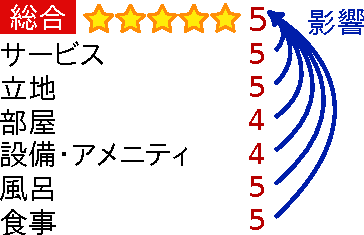
\includegraphics[0.3]{fig/relations_among_rating_categories.pdf}
  \caption{カテゴリ間の関係の例}
  \label{fig:RelationsAmongRatingCategories}
\end{figure}

しかし、個々のレビューに対して全ての文ベクトルを
ニューラルネットワークによる分類器の入力とすることは問題がある。
なぜならば、文の数はレビュー毎に異なっており、
複数レビュー内の複数の文ベクトルを単純な行列として表せないためである。
これは、分類器のミニバッチ方式の訓練を難しくし、
プログラムの実行時間を増加させる。
この問題に対処するため、本手法では各レビュー内の文ベクトルに対して
重み付け平均を行う。
これにより、全てのレビューで文ベクトルの数が統一され、
複数レビュー内の複数の文ベクトルをまとめて3次元行列として表すことができる。
つまり、ミニバッチ方式の訓練における計算が容易となる。

分類器はニューラルネットワークを用いて構成することによって、
文書・文間の関係とカテゴリ間の関係を同時に捉えた分類を行う。
従来手法\cite{nal14}や\cite{rie14}、\cite{duyu15}では、
単語ベクトルに対して畳込みニューラルネットワークが用いられている。
しかし、提案手法においては、畳み込みニューラルネットワークより
全結合ニューラルネットワークを用いた方が正答率が高かったため、
分類器には後者のみを用いた。


\subsection{アルゴリズム}

提案手法の処理の流れを説明する。
図\ref{fig:MyAlgorithm}にアルゴリズム全体の概略を示す。

\begin{figure}
  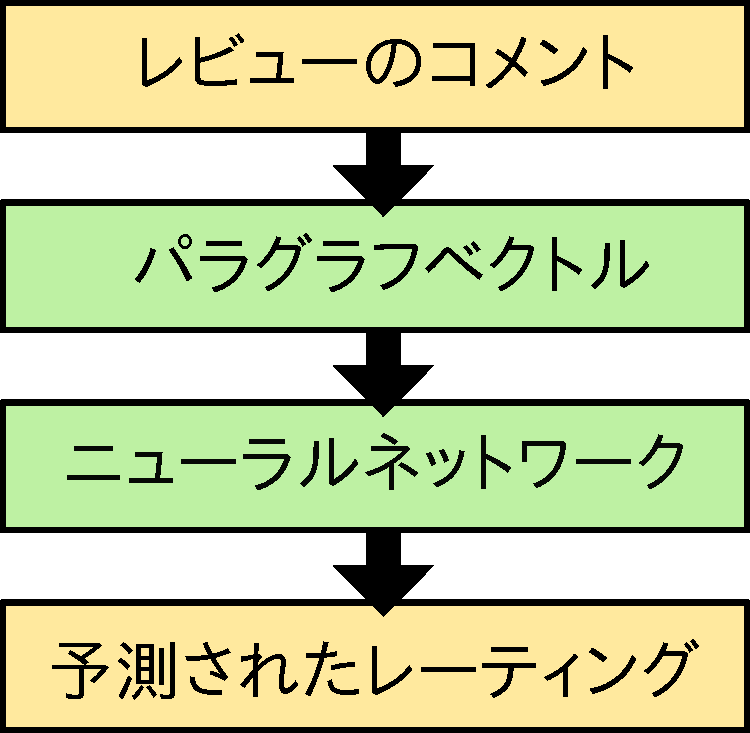
\includegraphics[0.5]{fig/algorithm.pdf}
  \caption{提案手法におけるアルゴリズムの概略}
  \label{fig:MyAlgorithm}
\end{figure}

%提案手法では、PV-DMによってレビュー内の文書全体及び各文の意味表現を
%生成し、それらをニューラルネットワークの入力として分類を行う。
%文毎の意味表現を用いることで文同士の位置関係を考慮し、
%ニューラルネットワークによる分類器を用いることで
%文間及びカテゴリ間の深い関係性を捉えることを目指す。
%提案手法の入力はレビューである文書と正解レーティングの組の集合、
%出力は各文書について予測されたカテゴリ毎のクラスである。
%以下に提案手法の処理の流れを示す。

初めに、PV-DMを用いて、
各レビューの文書全体のベクトルとそれに含まれる各文のベクトルを生成する。
以降、これらをそれぞれ文書ベクトル、文ベクトルと呼ぶ。
文書ベクトルと文ベクトルについては別々に学習し生成する。
%式\ref{eq:PVObjective}に示す目的関数$L_d$を最大化するように学習を行う。
%\begin{multline}
%  L_d = \sum^{T}_{t = n + 1} \{ \log \sigma(s(w_t, w_{t-n}, ..., w_{t-1}, d)) \\
%        + \sum^{k}_{w_{t}' \sim P_n}
%        \log(1 - \sigma(s(w_{t}', w_{t-n}, ..., w_{t-1}, d))) \},
%    \label{eq:PVObjective} \\
%\end{multline}
%\begin{gather}
%  s(w_t, w_{t - n}, ..., w_{t - 1}, d)
%    = W_{map}(w_t)
%      \cdot \begin{bmatrix} W(w_{t - n}) \\ \vdots
%      \\ W(w_{t - 1}) \\ D(d) \end{bmatrix} \nonumber
%\end{gather}
%ここで、$T$は現在の文章内の単語数、$t$は現在の単語位置、$d$は現在の文章、
%$w_i$は位置$i$にある単語、$n$はウィンドウサイズである。
%$W(w_i)$は単語$w_i$に相当する単語ベクトルを単語行列$W$から抜き出す関数を表す。
%$D(d)$は文章$d$に相当する文章ベクトルを文章行列$D$から抜き出す関数を表す。
%関数$s(w_t, w_0, ..., w_n, d)$はある単語とそれが出現する文脈との類似度を
%計算する。
%行列$W_{map}$は内積によって文脈と単語との類似度を計算するための単語毎
%のベクトルを保持する。
%文章行列内の各文章ベクトルはレビュー全体を表す文書ベクトル、または、
%各レビュー内の文ベクトルを表す。
%$\sigma$はシグモイド関数である。
%また、式\ref{eq:PVObjective}の中括弧内の右項はネガティブサンプリングを
%表す。
%ネガティブサンプリングとは、文脈外の単語をデータセットにおける出現確率で
%サンプリングし、それらと文脈の意味が遠ざかるように学習する手法である。
%$w_{t}' \sim P_n$は文脈外の単語$w_{t}'$を単語の出現頻度$P_n$によって
%サンプリングすることを示す。
%ただし、出現頻度は極端に頻出する単語の影響を抑えるため
%各単語に対して3/4乗している。
%現在の単語と同じ単語や同一回の学習で一度サンプリングされた単語は
%サンプリングしない。
式\ref{eq:ParagraphVector}の目的関数における$h$には
引数のベクトルを結合する関数を用いる。
また、学習の高速化のため、Quocら\cite{quoc14}によって
用いられている階層的softmax関数の代替として、ネガティブサンプリングを行う。
ネガティブサンプリングとは、文脈外の単語をデータセットにおける出現確率で
サンプリングし、それらと文脈の意味が遠ざかるように学習する手法である。
ただし、出現頻度は極端に頻出する単語の影響を抑えるため
各単語に対して3/4乗している。
現在の単語と同じ単語や同一回の学習で一度サンプリングされた単語は
サンプリングしない。

次に、各レビュー内の全ての文ベクトルに対して重み付け平均を行い、
圧縮された文ベクトルを生成する。
この過程により、各レビューで疎らだった文の数を統一する。
式\ref{eq:WeightedAverageSV}に重み付け平均によって圧縮した
文ベクトル$t_{i_{part}}$を示す。
各文ベクトルは圧縮後の各文ベクトルと位置が近いほど重みが大きくなるように
重み付け平均する。
\begin{gather}
  \mathbf{t}_{i_{part}} = \sum_{i_{sent}}
                          \frac{w(x_{i_{part}}(i_{sent}))}
                               {|\sum_{i_{sent}'} w(x_{i_{part}}(i_{sent}'))|}
                          \mathbf{s}_{i_{sent}},
  \label{eq:WeightedAverageSV} \\
  x_{i_{part}}(i_{sent}) = \frac{i_{sent} - i_{part}}{\#partitions},
  \nonumber \\
  w(x) = \begin{cases}
    \frac{1}{2} (\cos(\pi|x|) + 1) &\text{if $|x| \leq 1$} \\
    0 &\text{otherwise}
  \end{cases} \nonumber
\end{gather}
ここで、$i_{sent}$はレビュー内の文のインデックス、
$\#partitions$は重み付け平均された後の文ベクトルの数、
$i_{part}$は重み付け平均された後の文ベクトルのインデックス、
$\mathbf{s}_{i_{sent}}$は文ベクトルである。
\footnote{重み付けの関数には$\cos$関数の他に、
$x$に対して線形に重みを減少させるような関数や、
単純に文を区画毎に平均するような関数も考えられる。
区画毎に平均する関数は他の2つより正答率が低く、線形な関数と
$\cos$関数はほぼ同じ正答率を示したため、$\cos$関数を採用した。}

最後に、分類器によってレーティング予測を行う。
分類器は全結合ニューラルネットワークによって構成される。
図\ref{fig:MyModel}に各層の結合の様子を示す。
\begin{figure}[t!]
  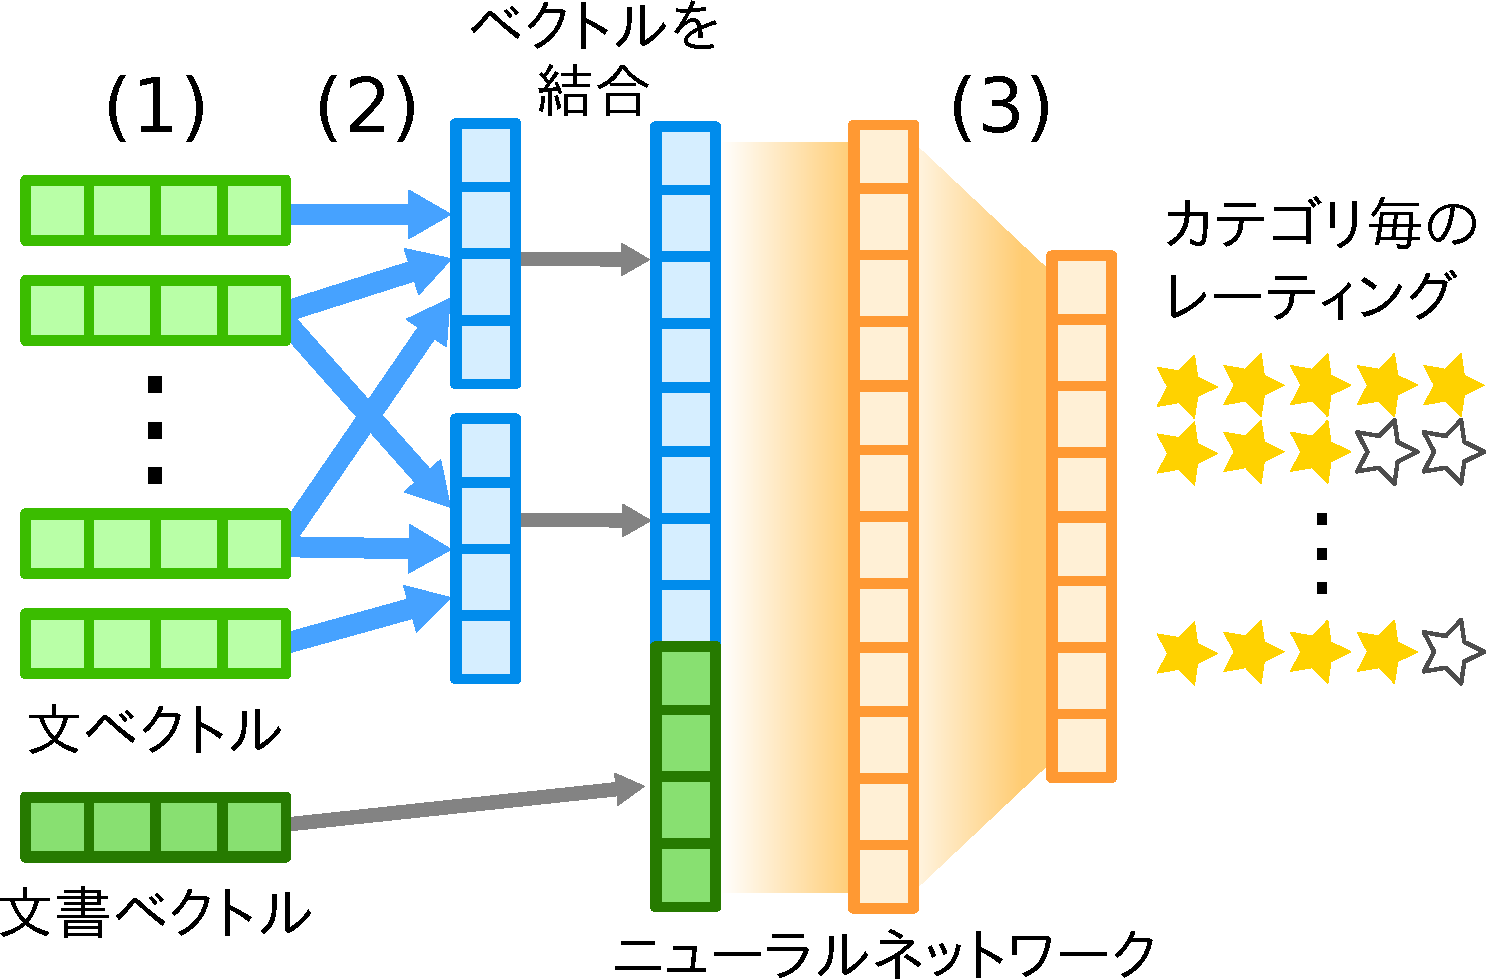
\includegraphics[0.6]{fig/model_with_formal_process_numbers.pdf}
  \caption{全結合ニューラルネットワークによる分類器}
  \label{fig:MyModel}
\end{figure}
入力層はレビュー毎の文書ベクトルと圧縮された文ベクトルの結合ベクトルである。
ニューラルネットワークの活性化関数には、シグモイド関数を用いる。
また、出力層はカテゴリの数とレーティングの場合の数の積だけのニューロンを持ち、
各ニューロンの出力はあるカテゴリ内であるレーティング値が選ばれることの
正規化されていない対数確率を表す。
ニューラルネットワークは式\ref{eq:NNObjective}に示す目的関数$E$を
最小化するように学習を行う。
\begin{gather}
  E = - \sum^{N}_{n = 1} \sum^{C}_{c = 1} \sum^{K}_{k = 1}
        d_{nck} \log{y_{ck}(x_n; w)},
  \label{eq:NNObjective} \\
  y_{ck}(x_n; w) = \frac{e^{u_{ck}(x_n; w)}}
                        {\sum^{K}_{j = 0} e^{u_{cj}(x_n; w)}} \nonumber
\end{gather}
各ニューロンの出力はカテゴリ毎に交差エントロピー誤差関数によって
損失に変換される。
ここで、$u_{ck}$は出力層のニューロンの出力値、$y_{ck}$はカテゴリ$c$において
クラス$k$が選ばれる確率、$w$はニューラルネットワークのパラメータである。
$d_{nck}$は$n$番目の文書がカテゴリ$c$でクラス$k$ならば1、
それ以外で0となる値である。
$N$はミニバッチサイズ、$C$はカテゴリの総数、$K$はクラスの総数である。

\section{実験} \label{sec:Experiments}

実験の目的は、提案手法のレーティング予測における優位性と、
提案手法に反映されている意図が実際にレーティング予測において有効であるかの
検証である。
具体的には、提案手法が従来手法\cite{fujitani15}に対して
優れているかを検証する。
また、提案手法を単純にした複数の比較手法を用意し、
提案手法がそれらより有意に優れていることを示す。
さらに、提案手法と比較手法及び比較手法同士の比較により、
文同士の位置関係の考慮や文書ベクトルと文ベクトルを同時に用いることが
レーティング予測に有効であるかを検証する。


\subsection{実験設定}

実験には、正答率を測定する実験と
提案手法における予測レーティングと正解レーティングのRMSEを
測定する実験の2つを行った。
比較手法として、提案手法における分類器の入力をそれぞれ
(1) DV (Document Vector)、
(2) ASV (Averaged Sentence Vector)、
(3) Weighted ASV
に変えた手法を用意した。
DVとはレビュー全体の文書ベクトルであり、
Quocら\cite{quoc14}の手法に相当する。
ASVとはレビュー内で平均した文ベクトルであり、
Weighted ASVとはレビュー内で重み付け平均によって圧縮された文ベクトルである。
Weighted ASVにおいて重み付け平均の方法は提案手法と同様であるが、
重み付け平均の式のハイパーパラメータは別に調整した。
有意差検定にはマクネマー検定を用い、p値が0.05より小さいとき有意とした。
また、RMSEの計算において正解または予測レーティングが0点であるものは
評価から省いた。
これは用いるデータセットのレビューにおいて、レーティングの0点は
レーティングが不可能であることを意味するためである。

データセットとしては、先行研究\cite{fujitani15}と同様に、
ホテル予約サイト楽天トラベルにおけるレビュー337,266件からレビューの番号順に
訓練データ300,000件、開発データ10,000件、評価データ10,000件を用いた。
楽天トラベルによって提供されている元のレビューデータは
レーティングを含むファイルとレビューの文書を含むファイルとに分かれている。
それぞれTab Separated Values (TSV)フォーマットで1行1レビューとして情報が
記述されている。
レーティングを含むファイルと文書を含むファイルのフォーマットを
それぞれ図\ref{fig:RatingFileFormat}と図\ref{fig:DocumentFileFormat}に示す。
以下に、それぞれのファイルから実験のために抽出した情報と
それらの前処理について記述する。
まず、レーティングを含むファイルからは、レビューのIDと
「立地」から「総合」カテゴリまでのレーティングを取り出した。
レビューの文書を含むファイルからは、レビューのIDと
レビューの文書を取り出した。
ただし、元のレビューの文書に含まれる「【ご利用の宿泊プラン】」以降の文字列は
ユーザが記述したものではないため取り除いた。
その後、レーティングとレビューの文書をレビューIDが一致するように組にした。
このとき、レーティングを含むファイル、または、レビューの文書を含むファイルの
どちらかにしか存在しないレビューIDを持つレビューは取り除いた。

\begin{figure}
  第1フィールド(レビューのID){[Tab]}第2フィールド{[Tab]} ... \\
  第7フィールド(「立地」カテゴリのレーティング){[Tab]} ... \\
  第13フィールド(「総合」カテゴリのレーティング)
  \caption{レーティングを含むTSVファイルのフォーマット}
  \label{fig:RatingFileFormat}
\end{figure}

\begin{figure}
  第1フィールド{[Tab]}第2フィールド(レビューの文書){[Tab]} \\
  第3フィールド(レビューのID){[Tab]} ...
  \caption{文書を含むTSVファイルのフォーマット}
  \label{fig:DocumentFileFormat}
\end{figure}

レビューの文書に対する前処理について以下に示す。
まず、全てのレビューの文書に対して文字コードをUTF-8に変換し、
以下の正規化処理を行った。
記号「!”#$%&’()*+,−./:;<>?@[¥]^_`{|}
\unicode{301C}」は全てNFKC形式で正規化した。
記号「\unicode{02D7}\unicode{058A}\unicode{2011}\unicode{2012}\unicode{2013}
\unicode{2043}\unicode{207B}\unicode{208B}\unicode{2212}」
は全て記号「-」で置き換えた。
記号「\unicode{FE63}-ー—―─━ー」は全て記号「ー」で置き換えた。
チルダ記号「\unicode{007E}\unicode{223C}\unicode{223E}\unicode{301C}
\unicode{3030}\unicode{FF5E}」は全て削除した。
ここで、\unicode{XXXX}は16進数で表現されたUnicodeのコードポイントを示す。
次に、各レビューの文書を文に分割した。
「。」、「.」、「!」、「?」を文の終端文字とし、
文の終端文字でない文字の1回より多い繰り返しと
文の終端文字または文書の終端の連続を
一つの文として正規表現によって解析した。
ただし、文が1つも解析できなかった文書については、
文書全体の文字列をその文書に含まれる唯一の文とした。
最後に、形態素解析には形態素解析器MeCabを用いた、
辞書にはIPA辞書を用いた。
単語の情報は表層のみを利用し、MeCabによって出力される
表層が無い特殊な単語は取り除いた。

表\ref{tab:ParametersOfMethods}に各手法におけるニューラルネットワークの
パラメータ設定を示す。
全ての手法において、中間層の数は1、入力層及び中間層におけるドロップアウト率は
それぞれ0.2と0.5で共通である。
Adam\cite{diederik15}のハイパーパラメータは\cite{diederik15}と同様の値を
用いた。
Weighted ASVと提案手法において圧縮された文ベクトルの数は
それぞれ3つと2つとした。
全ての実験において文書及び文ベクトルについては、
学習回数は1,024回、学習する単語の範囲は前3単語、単語の最少出現回数は5回、
ネガティブサンプリングの回数は5回、ベクトルの次元数は600次元に
設定し学習したものを用いた。

\begin{table}
  \caption{各手法のパラメータ設定}
  \centering
  \begin{tabular}{l | r r} \label{tab:ParametersOfMethods}
    手法 & 学習回数 & 中間層でのユニット数 \\
    \hline
    DV & 20 & 512 \\
    ASV & 55 & 256 \\
    Weighted ASV & 24 & 256 \\
    提案手法 & 30 & 512 \\
  \end{tabular}
\end{table}


\subsection{結果}

まず、提案手法と3つの比較手法、従来手法\cite{fujitani15}を
正答率で比較したものを表\ref{tab:AccuraciesOfMethods}に示す。
また、表\ref{tab:AccuraciesPerCategory}に提案手法と
従来手法\cite{fujitani15}におけるカテゴリ別の正答率を示す。
そのグラフを図\ref{tab:AccuraciesPerCategory}に示す。
表\ref{tab:AccuraciesOfMethods}において、
提案手法が従来手法\cite{fujitani15}の正答率を0.0198有意に上回っている。
また、提案手法がDVとWeighted ASVの正答率をそれぞれ0.0050と0.0163
有意に上回っている。
Weighted ASVがASVを0.0029有意に上回っている。

\begin{table}
  \caption{各手法における正答率}
  \centering
  \begin{tabular}{l | r} \label{tab:AccuraciesOfMethods}
    手法 & 正答率 \\
    \hline
    従来手法\cite{fujitani15} & 0.4832 \\
    DV & 0.4980 \\
    ASV & 0.4838 \\
    Weighted ASV & 0.4867 \\
    提案手法 & \textbf{0.5030} \\
  \end{tabular}
\end{table}

\begin{table}
  \caption{提案手法と従来手法\cite{fujitani15}におけるカテゴリ別の正答率}
  \centering
  \begin{tabular}{r | r r r r r r r} \label{tab:AccuraciesPerCategory}
    手法 & 立地 & 部屋 & 食事 & 風呂 & サービス & 設備 & 総合 \\
    \hline
    従来手法\cite{fujitani15}
        & 0.4961 & 0.4706 & 0.5140 & 0.3973 & 0.4783 & 0.4265 & 0.5660 \\
    提案手法 & 0.5140 & 0.4984 & 0.5353 & 0.4347 & 0.5116 & 0.4479 & 0.5794 \\
  \end{tabular}
\end{table}

次に、表\ref{tab:RMSEsPerCategory}にレーティングのRMSEを測定した結果を示す。
そのグラフを図\ref{tab:RMSEsPerCategory}に示す。
提案手法は従来手法\cite{fujitani15}が欠点としていた
食事と風呂のカテゴリにおいてそれぞれ0.65及び0.34だけ低い誤差を示した。
また、その他全てのカテゴリにおいても提案手法は従来手法より低い誤差を示した。

\begin{table}
  \caption{提案手法と従来手法\cite{fujitani15}におけるカテゴリ別の
           レーティングのRMSE}
  \centering
  \begin{tabular}{r | r r r r r r r} \label{tab:RMSEsPerCategory}
    手法 & 立地 & 部屋 & 食事 & 風呂 & サービス & 設備 & 総合 \\
    \hline
    従来手法\cite{fujitani15}
        & 0.97 & 0.97 & 1.53 & 1.27 & 0.94 & 0.95 & 0.81 \\
    提案手法 & 0.88 & 0.88 & 0.93 & 1.03 & 0.86 & 0.90 & 0.73 \\
  \end{tabular}
\end{table}

最後に、正答率を測定する実験における、提案手法の精度と再現率、F値を
それぞれ表\ref{tab:ProposedMethodPrecision}と
表\ref{tab:ProposedMethodRecall}、表\ref{tab:ProposedMethodFValue}に示す。
表においてN/Aは計算不可能であることを示す。
また、カテゴリ毎の正解レーティングの内訳と
提案手法のカテゴリ毎の予測レーティングの内訳を
表\ref{tab:AnswerRatings}と表\ref{tab:PredictedRatings}に示す。

\begin{table}
  \caption{提案手法の精度}
  \centering
  \begin{tabular}{r | r r r r r r r | r} \label{tab:ProposedMethodPrecision}
    レーティング & 立地 & 部屋 & 食事 & 風呂 & サービス & 設備 & 総合
      & 全カテゴリ \\
    \hline
    \csvreader[no head,late after line=\\]
      {csv/class_precision.csv}
      {1=\rating,2=\location,3=\room,4=\mean,5=\bath,6=\service,7=\facilities,
       8=\overall,9=\allcategories}
      {\rating & \location & \room & \mean & \bath & \service & \facilities
       & \overall & \allcategories}
  \end{tabular}
\end{table}

\begin{table}
  \caption{提案手法の再現率}
  \centering
  \begin{tabular}{r | r r r r r r r | r} \label{tab:ProposedMethodRecall}
    レーティング & 立地 & 部屋 & 食事 & 風呂 & サービス & 設備 & 総合
      & 全カテゴリ \\
    \hline
    \csvreader[no head,late after line=\\]
      {csv/class_recall.csv}
      {1=\rating,2=\location,3=\room,4=\mean,5=\bath,6=\service,7=\facilities,
       8=\overall,9=\allcategories}
      {\rating & \location & \room & \mean & \bath & \service & \facilities
       & \overall & \allcategories}
  \end{tabular}
\end{table}

\begin{table}
  \caption{提案手法のF値}
  \centering
  \begin{tabular}{r | r r r r r r r | r} \label{tab:ProposedMethodFValue}
    レーティング & 立地 & 部屋 & 食事 & 風呂 & サービス & 設備 & 総合
      & 全カテゴリ \\
    \hline
    \csvreader[no head,late after line=\\]
      {csv/class_f_value.csv}
      {1=\rating,2=\location,3=\room,4=\mean,5=\bath,6=\service,7=\facilities,
       8=\overall,9=\allcategories}
      {\rating & \location & \room & \mean & \bath & \service & \facilities
       & \overall & \allcategories}
  \end{tabular}
\end{table}

\begin{table}
  \caption{カテゴリ毎の正解レーティング件数}
  \centering
  \begin{tabular}{r | r r r r r r r | r} \label{tab:AnswerRatings}
    レーティング & 立地 & 部屋 & 食事 & 風呂 & サービス & 設備 & 総合
      & 全カテゴリ \\
    \hline
    \csvreader[no head,late after line=\\]
      {csv/answer_class_count.csv}
      {1=\rating,2=\location,3=\room,4=\mean,5=\bath,6=\service,7=\facilities,
       8=\overall,9=\allcategories}
      {\rating & \location & \room & \mean & \bath & \service & \facilities
       & \overall & \allcategories}
  \end{tabular}
\end{table}

\begin{table}
  \caption{提案手法のカテゴリ毎の予測レーティング件数}
  \centering
  \begin{tabular}{r | r r r r r r r | r} \label{tab:PredictedRatings}
    レーティング & 立地 & 部屋 & 食事 & 風呂 & サービス & 設備 & 総合
      & 全カテゴリ \\
    \hline
    \csvreader[no head,late after line=\\]
      {csv/predicted_class_count.csv}
      {1=\rating,2=\location,3=\room,4=\mean,5=\bath,6=\service,7=\facilities,
       8=\overall,9=\allcategories}
      {\rating & \location & \room & \mean & \bath & \service & \facilities
       & \overall & \allcategories}
  \end{tabular}
\end{table}

\begin{figure}
  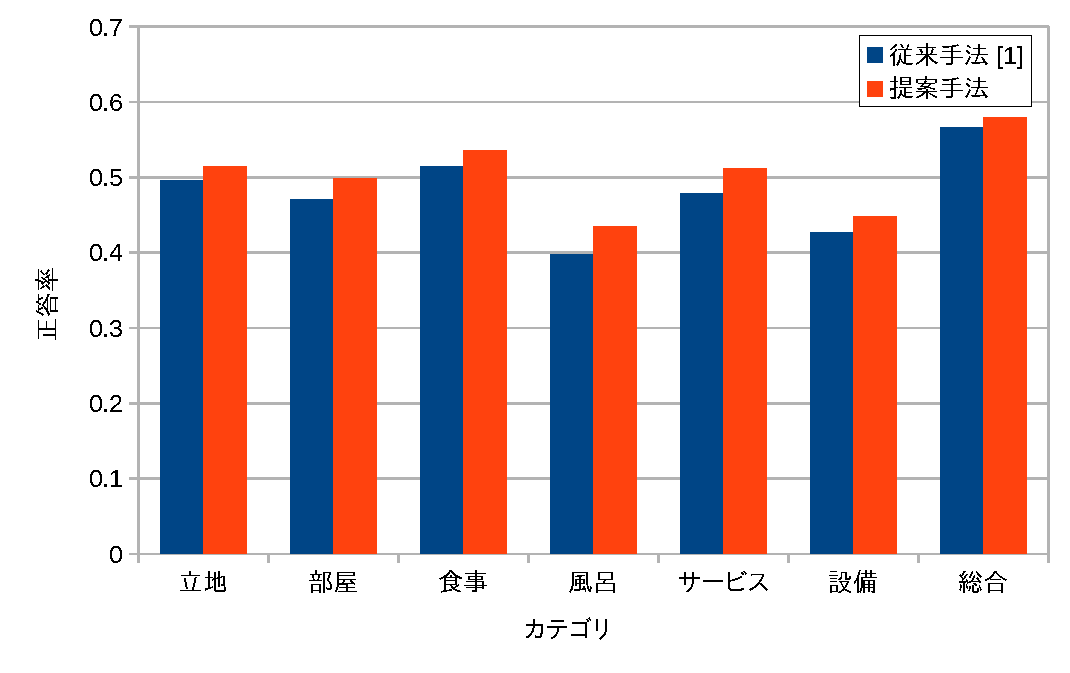
\includegraphics{fig/graph_of_accuracies_per_category.pdf}
  \caption{提案手法と従来手法\cite{fujitani15}におけるカテゴリ別の正答率}
  \label{fig:AccuraciesPerCategory}
\end{figure}

\begin{figure}
  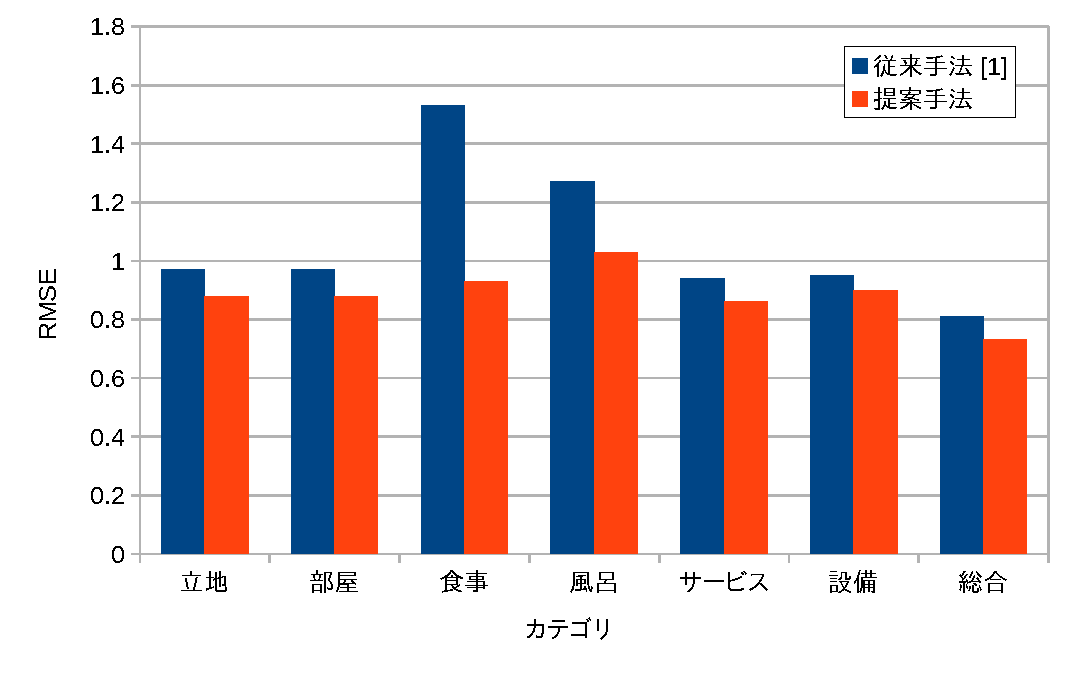
\includegraphics{fig/graph_of_rmses_per_category.pdf}
  \caption{提案手法と従来手法\cite{fujitani15}におけるカテゴリ別の
           レーティングのRMSE}
  \label{fig:RMSEsPerCategory}
\end{figure}

\section{考察} \label{sec:Discussion}

%実験結果より、提案手法と3つの比較手法全てが従来手法の正答率を上回っている。
提案手法が従来手法\cite{fujitani15}の正答率を
0.0198有意に上回っていることから、提案手法が従来手法\cite{fujitani15}より
正答率において優れていることが分かった。
また、Weighted ASVの正答率がASVの正答率を0.0029有意に上回っていることから、
文の位置関係の考慮がレーティング予測に有効であることが分かった。
さらに、提案手法がWeighted ASVに比べ有意に高い正答率を示していることから、
文書ベクトルと文ベクトルを同時に特徴量として用いることがレーティング予測に
有効であることが分かった。
これは文書ベクトルと文ベクトルがいくらか異なる特徴を学習していることを示す。

藤谷ら\cite{fujitani15}より、実験で用いたデータセットには、
食事のカテゴリにおいて0点が付与されたレビューが108,079件存在する。
また、風呂のカテゴリでは13,332件、設備のカテゴリでは2,011件存在し、
他のカテゴリでは0件である。
一般に、0点はユーザが何らかの理由でレーティング不可能と判断したことを示す。
例えば、「食事」のカテゴリならばホテルで食事を取っていない、
「風呂」のカテゴリならば別の入浴施設を利用した等である。
よって、提案手法は従来手法\cite{fujitani15}よりレビュー中の上記のような意味を
よく捉えていると考えられる。

次に、提案手法の問題点について考察する。
提案手法の問題点の一つは、レビューの素性の生成と分類のモデルが
分離していることである。
具体的には、PV-DMによってレビューの文書とそれが含む文の素性を生成する段階、
及び、それらをニューラルネットワークによって分類を行う段階の2つに分離している。
このことは、問題を2つに分けることで個々の問題を単純にしているが、
同時にいくつかの問題を伴う。
1つ目は、レビューを一つずつレーティング予測することができないことである。
提案手法では、新しいレビューを訓練データに加える場合、
全てのレビューの文書・文ベクトルを再構築する必要がある。
レビューの件数が多い場合、これは大量の計算を必要とし効率的ではない。
これは提案手法が実際に応用されるときに問題となる。
なぜなら、実際の商品レビューの件数は時間と共に増加していくためである。
2つ目は、文書や文の素性やそれらを生成するモデルのパラメータが分類時に
調整できないことである。
最大の正答率を達成するためには、これらは分類器のパラメータと同様に
分類問題に対して最適化されることが望ましい。
3つ目は、単語間の関係が分類時に十分に考慮できないことである。
単語間の関係は文書・文ベクトルによって表現されているが、
それらは分類の正答率が最大になるように表現されているとは限らない。
以上より、提案手法の素性の生成と分類のモデルは統合するべきである。

\section{結論}

本研究では、多カテゴリにおける評判分類問題について、
レビュー全体の文書ベクトルに加え重み付け平均された文ベクトルを用いた手法を
提案した。

実験では、提案手法が従来手法\cite{fujitani15}より高い正答率を示した。
また、比較手法の結果より、
レビュー内の文の並びが評判分類に重要であること、及び、
文書ベクトルと文ベクトルがレビューのいくらか異なる特徴を捉えていることが
分かった。

今後の課題は言語要素間のより多様で複雑な関係を考慮することである。
このためには、各レビューの意味表現を生成するモデルと
分類を行うモデルを1つに統合する必要がある。
なぜならば、モデルが分かれていることによって
単語や文字などのより小さな言語要素同士の関係を分類時に考慮できないためである。
モデルの統合によって、学習手法の柔軟性を高めると共に
さらなる正答率の向上を目指す。


%今後の課題は、提案手法の中で2つに分かれているモデルの統合である。
%
%提案手法は、分類すべき文書とそれが含む文の分散表現を生成する段階、及び、
%それらを用いて分類を行う段階の2つの段階に分かれている。
%このことは、問題を2つに分けることで個々の問題を単純にしているが、
%同時に文書の分類を一つずつ行うことを難しくしている。
%また、文書や文の分散表現を事前に生成するための
%PV-DMのパラメータは、実際には最大の正答率を達成するため
%分類器のパラメータとして最適化されることが望ましい。
%
%今後は、これらの問題を解決するために、文書や文の分散表現を生成する過程を
%ニューラルネットワークによる分類器に統合する。
%これによって、学習方法の柔軟性を高めると共にさらなる正答率の向上を目指す。


\section*{謝辞}

本研究を進めるにあたって、佐々木裕教授、三輪誠准教授に御指導いただきました。
同研究室の先輩方、友人には多くの協力、助言をいただきました。
また、本研究の実験において、楽天株式会社より
ホテル予約サイト楽天トラベルにおけるレビューデータを使用させていただきました。
この場を借りて感謝致します。

\bibliographystyle{jplain}
\begin{thebibliography}{9}
\bibitem{fujitani15}
  藤谷宣典ら,
  隠れ状態を用いたホテルレビューのレーティング予測.
  言語処理学会第21回年次大会, 2015.
\bibitem{quoc14}
  Quoc Le et al.,
  Distributed Representations of Sentences and Documents.
  ICML 2014, 2014.
\bibitem{nal14}
  Nal Kalchbrenner et al.,
  A Convolutional Neural Network for Modelling Sentences.
  ACL 2014, 2014.
\bibitem{rie14}
  Rie Johnson et al.,
  Effective Use of Word Order for Text Categorization
  with Convolutional Neural Networks.
  NAACL 2015, 2015.
\bibitem{duyu15}
  Duyu Tang et al.,
  Learning Semantic Representation of Users and Products
  for Document Level Sentiment Classification.
  ACL 2015, 2015.
\bibitem{yoshua03}
  Yoshua Bengio et al.,
  A Neural Probabilistic Language Model.
  The Journal of Machine Learning Research 3, 2003.
\bibitem{mihai12}
  Mihai Surdeanu et al.,
  Multi-instance Multi-label Learning for Relation Extraction.
  CoNLL 2012, 2012.
\bibitem{diederik15}
  Diederik Kingma et al.,
  Adam: A Method for Stochastic Optimization.
  ICLR 2015, 2015.
\bibitem{john12}
  John Duchi et al.,
  Adaptive Subgradient Methods for Online Learning and Stochastic Optimization.
  Journal of Machine Learning Research 12, 2011.
\bibitem{hozumi06}
  田中穂積,
  自然言語処理 -基礎と応用-.
  電子情報通信学会.
\bibitem{takayuki2015}
  岡谷貴之,
  深層学習.
  講談社.
\end{thebibliography}


\end{document}
